\documentclass{beamer}
\usepackage{graphicx}
\usepackage{numprint}
\usepackage{minted}
\usepackage{color}
\usepackage{hyperref}
\usepackage[norsk]{babel}
\usepackage{lipsum}

\newminted{json}{fontsize=\scriptsize,
    linenos,
    numbersep=8pt,
    gobble=4,
    frame=lines,
    bgcolor=bg,
    framesep=3mm}

\newminted{kotlin}{fontsize=\scriptsize,
    linenos,
    numbersep=8pt,
    gobble=4,
    frame=lines,
    bgcolor=bg,
    framesep=3mm}

\newminted{zsh}{fontsize=\scriptsize,
    linenos,
    numbersep=8pt,
    gobble=12,
    frame=lines,
    bgcolor=bg,
    framesep=3mm}


\hypersetup{
    colorlinks   = true,    % Colours links instead of ugly boxes
    urlcolor     = blue,    % Colour for external hyperlinks
    linkcolor    = blue,    % Colour of internal links
    citecolor    = red,      % Colour of citations
%    bookmarksopen,
%    bookmarksnumbered,
}


%Information to be included in the title page:
\title{GIT}
\subtitle{To the core}
\author{\href{kjetil.nygard@tietoevry.com}{Kjetil Nygård}}
\institute{TietoEvry}
\date{Torsdag 23. Februar 2023}

\usetheme{Warsaw}
\usecolortheme{default}


\begin{document}

    \frame{\titlepage}


    %%%%%%%%%%%%%%%%%%%%%%%%%%%%%%%%%%%%%%%%%%%%%%%%%%%%%%%%%%%%%%%%%%%%%%%%%%%%%%%%%%%%%%
    % What is GIT
    %%%%%%%%%%%%%%%%%%%%%%%%%%%%%%%%%%%%%%%%%%%%%%%%%%%%%%%%%%%%%%%%%%%%%%%%%%%%%%%%%%%%%%
    \begin{frame}
        \frametitle{What is GIT}
        \begin{columns}[c]
            \begin{column}{.55\textwidth}
                \begin{block}{Definisjon}
                    Git is a distributed version control system that tracks changes
                    in any set of computer files.
                \end{block}
                \begin{block}{Content}
                    \begin{enumerate}
                        \item Workflows
                        \item Datastruktur
                        \item .git folderen
                        \item Kommandoer
                    \end{enumerate}
                \end{block}
            \end{column}
            \begin{column}{.45\textwidth}
                \begin{center}
                    
\includegraphics[width=\textwidth]{images/Git-Logo-2Color}
                \end{center}
            \end{column}
        \end{columns}
    \end{frame}


    %%%%%%%%%%%%%%%%%%%%%%%%%%%%%%%%%%%%%%%%%%%%%%%%%%%%%%%%%%%%%%%%%%%%%%%%%%%%%%%%%%%%%%
    % Commits
    %%%%%%%%%%%%%%%%%%%%%%%%%%%%%%%%%%%%%%%%%%%%%%%%%%%%%%%%%%%%%%%%%%%%%%%%%%%%%%%%%%%%%%
    \begin{frame}
        \frametitle{Local development}
        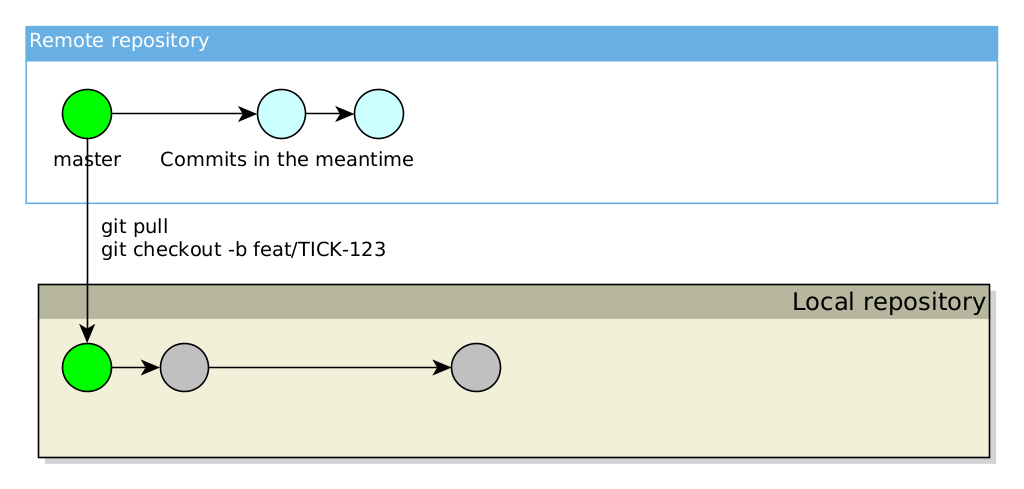
\includegraphics[width=\textwidth]{images/git-commits/01-work-phase}
    \end{frame}


    %%%%%%%%%%%%%%%%%%%%%%%%%%%%%%%%%%%%%%%%%%%%%%%%%%%%%%%%%%%%%%%%%%%%%%%%%%%%%%%%%%%%%%
    % Merge workflow
    %%%%%%%%%%%%%%%%%%%%%%%%%%%%%%%%%%%%%%%%%%%%%%%%%%%%%%%%%%%%%%%%%%%%%%%%%%%%%%%%%%%%%%
    \begin{frame}
        \frametitle{Merge workflow}
        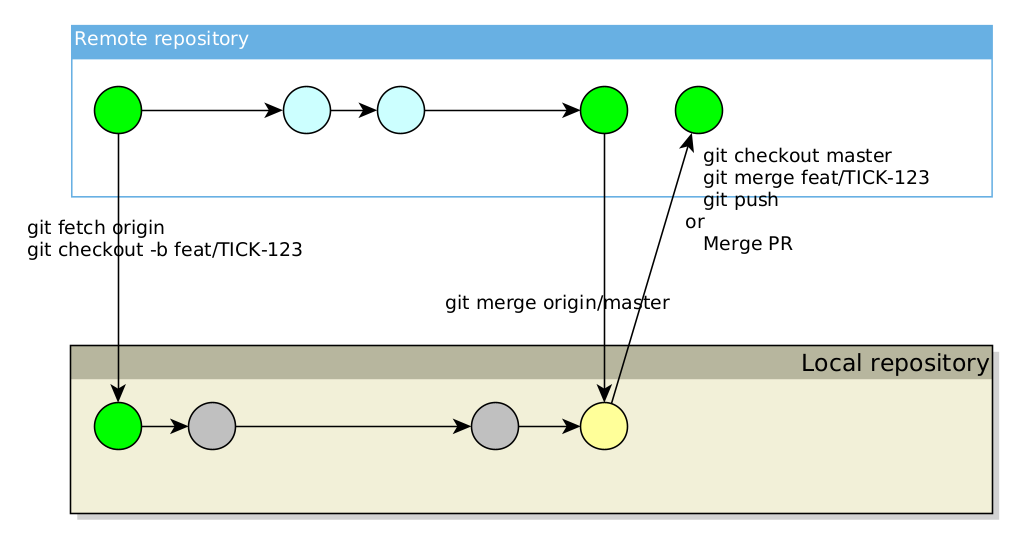
\includegraphics[width=\textwidth]{images/git-commits/10-merge-workflow}
    \end{frame}


    %%%%%%%%%%%%%%%%%%%%%%%%%%%%%%%%%%%%%%%%%%%%%%%%%%%%%%%%%%%%%%%%%%%%%%%%%%%%%%%%%%%%%%
    % Rebase workflow
    %%%%%%%%%%%%%%%%%%%%%%%%%%%%%%%%%%%%%%%%%%%%%%%%%%%%%%%%%%%%%%%%%%%%%%%%%%%%%%%%%%%%%%
    \begin{frame}
        \frametitle{Rebase workflow}
        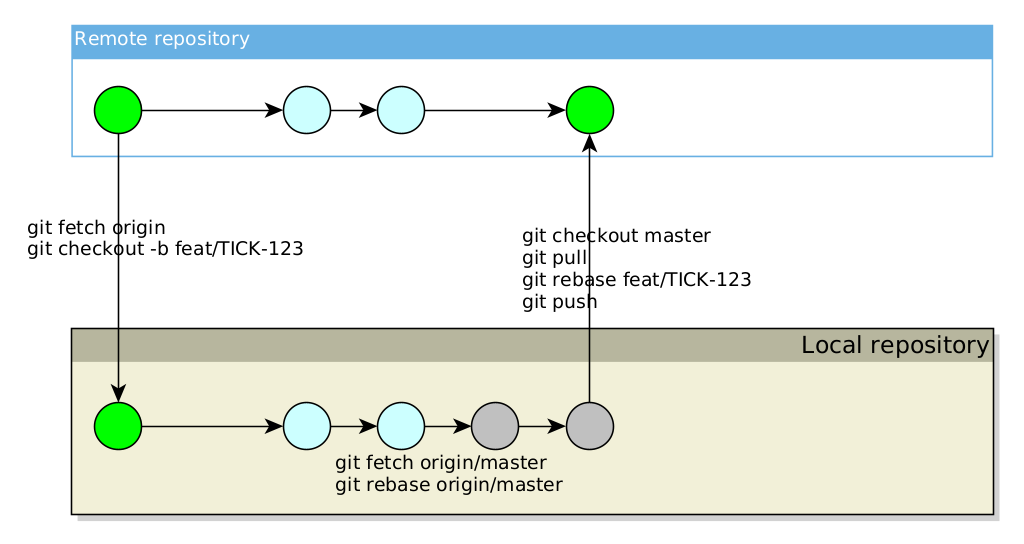
\includegraphics[width=\textwidth]{images/git-commits/20-rebase-workflow}
    \end{frame}


    %%%%%%%%%%%%%%%%%%%%%%%%%%%%%%%%%%%%%%%%%%%%%%%%%%%%%%%%%%%%%%%%%%%%%%%%%%%%%%%%%%%%%%
    % Datastructure
    %%%%%%%%%%%%%%%%%%%%%%%%%%%%%%%%%%%%%%%%%%%%%%%%%%%%%%%%%%%%%%%%%%%%%%%%%%%%%%%%%%%%%%
    \begin{frame}
        \frametitle{Git datastructure}
        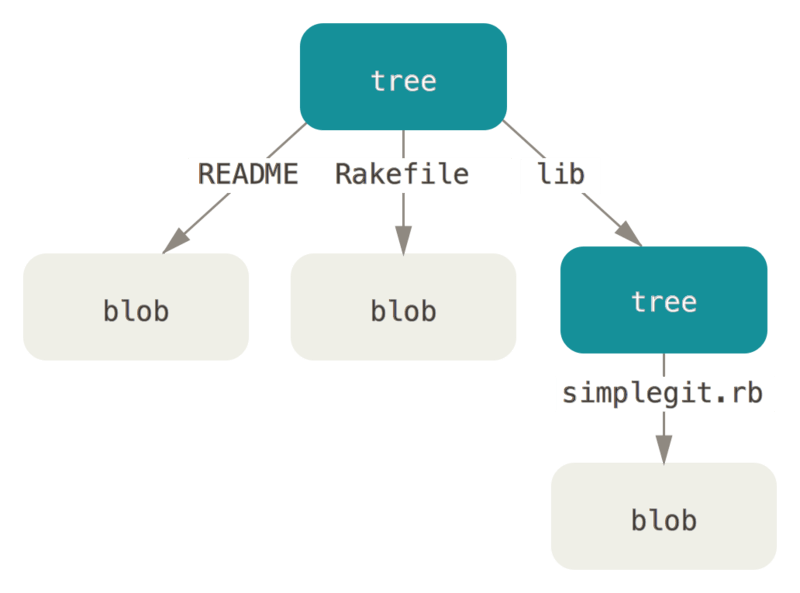
\includegraphics[width=\textwidth]{images/git-data-model-1}
    \end{frame}


    %%%%%%%%%%%%%%%%%%%%%%%%%%%%%%%%%%%%%%%%%%%%%%%%%%%%%%%%%%%%%%%%%%%%%%%%%%%%%%%%%%%%%%
    % Commands
    %%%%%%%%%%%%%%%%%%%%%%%%%%%%%%%%%%%%%%%%%%%%%%%%%%%%%%%%%%%%%%%%%%%%%%%%%%%%%%%%%%%%%%
    \begin{frame}
        \frametitle{Commands}

        \begin{block}{Content}
            \begin{enumerate}
                \item git reset --hard
                \item git log --numstat
                \item git reflog
                \item git grep
                \item git cat-file -p
                \item git diff
                \item gir rm
            \end{enumerate}
        \end{block}

    \end{frame}


    %%%%%%%%%%%%%%%%%%%%%%%%%%%%%%%%%%%%%%%%%%%%%%%%%%%%%%%%%%%%%%%%%%%%%%%%%%%%%%%%%%%%%%
    % The End
    %%%%%%%%%%%%%%%%%%%%%%%%%%%%%%%%%%%%%%%%%%%%%%%%%%%%%%%%%%%%%%%%%%%%%%%%%%%%%%%%%%%%%%
    \begin{frame}
        \frametitle{Thank you for your attention}
        Spørsmål?
    \end{frame}

\end{document}